% Options for packages loaded elsewhere
% Options for packages loaded elsewhere
\PassOptionsToPackage{unicode}{hyperref}
\PassOptionsToPackage{hyphens}{url}
\PassOptionsToPackage{dvipsnames,svgnames,x11names}{xcolor}
%
\documentclass[
  letterpaper,
  DIV=11,
  numbers=noendperiod]{scrartcl}
\usepackage{xcolor}
\usepackage{amsmath,amssymb}
\setcounter{secnumdepth}{-\maxdimen} % remove section numbering
\usepackage{iftex}
\ifPDFTeX
  \usepackage[T1]{fontenc}
  \usepackage[utf8]{inputenc}
  \usepackage{textcomp} % provide euro and other symbols
\else % if luatex or xetex
  \usepackage{unicode-math} % this also loads fontspec
  \defaultfontfeatures{Scale=MatchLowercase}
  \defaultfontfeatures[\rmfamily]{Ligatures=TeX,Scale=1}
\fi
\usepackage{lmodern}
\ifPDFTeX\else
  % xetex/luatex font selection
\fi
% Use upquote if available, for straight quotes in verbatim environments
\IfFileExists{upquote.sty}{\usepackage{upquote}}{}
\IfFileExists{microtype.sty}{% use microtype if available
  \usepackage[]{microtype}
  \UseMicrotypeSet[protrusion]{basicmath} % disable protrusion for tt fonts
}{}
\makeatletter
\@ifundefined{KOMAClassName}{% if non-KOMA class
  \IfFileExists{parskip.sty}{%
    \usepackage{parskip}
  }{% else
    \setlength{\parindent}{0pt}
    \setlength{\parskip}{6pt plus 2pt minus 1pt}}
}{% if KOMA class
  \KOMAoptions{parskip=half}}
\makeatother
% Make \paragraph and \subparagraph free-standing
\makeatletter
\ifx\paragraph\undefined\else
  \let\oldparagraph\paragraph
  \renewcommand{\paragraph}{
    \@ifstar
      \xxxParagraphStar
      \xxxParagraphNoStar
  }
  \newcommand{\xxxParagraphStar}[1]{\oldparagraph*{#1}\mbox{}}
  \newcommand{\xxxParagraphNoStar}[1]{\oldparagraph{#1}\mbox{}}
\fi
\ifx\subparagraph\undefined\else
  \let\oldsubparagraph\subparagraph
  \renewcommand{\subparagraph}{
    \@ifstar
      \xxxSubParagraphStar
      \xxxSubParagraphNoStar
  }
  \newcommand{\xxxSubParagraphStar}[1]{\oldsubparagraph*{#1}\mbox{}}
  \newcommand{\xxxSubParagraphNoStar}[1]{\oldsubparagraph{#1}\mbox{}}
\fi
\makeatother

\usepackage{color}
\usepackage{fancyvrb}
\newcommand{\VerbBar}{|}
\newcommand{\VERB}{\Verb[commandchars=\\\{\}]}
\DefineVerbatimEnvironment{Highlighting}{Verbatim}{commandchars=\\\{\}}
% Add ',fontsize=\small' for more characters per line
\usepackage{framed}
\definecolor{shadecolor}{RGB}{241,243,245}
\newenvironment{Shaded}{\begin{snugshade}}{\end{snugshade}}
\newcommand{\AlertTok}[1]{\textcolor[rgb]{0.68,0.00,0.00}{#1}}
\newcommand{\AnnotationTok}[1]{\textcolor[rgb]{0.37,0.37,0.37}{#1}}
\newcommand{\AttributeTok}[1]{\textcolor[rgb]{0.40,0.45,0.13}{#1}}
\newcommand{\BaseNTok}[1]{\textcolor[rgb]{0.68,0.00,0.00}{#1}}
\newcommand{\BuiltInTok}[1]{\textcolor[rgb]{0.00,0.23,0.31}{#1}}
\newcommand{\CharTok}[1]{\textcolor[rgb]{0.13,0.47,0.30}{#1}}
\newcommand{\CommentTok}[1]{\textcolor[rgb]{0.37,0.37,0.37}{#1}}
\newcommand{\CommentVarTok}[1]{\textcolor[rgb]{0.37,0.37,0.37}{\textit{#1}}}
\newcommand{\ConstantTok}[1]{\textcolor[rgb]{0.56,0.35,0.01}{#1}}
\newcommand{\ControlFlowTok}[1]{\textcolor[rgb]{0.00,0.23,0.31}{\textbf{#1}}}
\newcommand{\DataTypeTok}[1]{\textcolor[rgb]{0.68,0.00,0.00}{#1}}
\newcommand{\DecValTok}[1]{\textcolor[rgb]{0.68,0.00,0.00}{#1}}
\newcommand{\DocumentationTok}[1]{\textcolor[rgb]{0.37,0.37,0.37}{\textit{#1}}}
\newcommand{\ErrorTok}[1]{\textcolor[rgb]{0.68,0.00,0.00}{#1}}
\newcommand{\ExtensionTok}[1]{\textcolor[rgb]{0.00,0.23,0.31}{#1}}
\newcommand{\FloatTok}[1]{\textcolor[rgb]{0.68,0.00,0.00}{#1}}
\newcommand{\FunctionTok}[1]{\textcolor[rgb]{0.28,0.35,0.67}{#1}}
\newcommand{\ImportTok}[1]{\textcolor[rgb]{0.00,0.46,0.62}{#1}}
\newcommand{\InformationTok}[1]{\textcolor[rgb]{0.37,0.37,0.37}{#1}}
\newcommand{\KeywordTok}[1]{\textcolor[rgb]{0.00,0.23,0.31}{\textbf{#1}}}
\newcommand{\NormalTok}[1]{\textcolor[rgb]{0.00,0.23,0.31}{#1}}
\newcommand{\OperatorTok}[1]{\textcolor[rgb]{0.37,0.37,0.37}{#1}}
\newcommand{\OtherTok}[1]{\textcolor[rgb]{0.00,0.23,0.31}{#1}}
\newcommand{\PreprocessorTok}[1]{\textcolor[rgb]{0.68,0.00,0.00}{#1}}
\newcommand{\RegionMarkerTok}[1]{\textcolor[rgb]{0.00,0.23,0.31}{#1}}
\newcommand{\SpecialCharTok}[1]{\textcolor[rgb]{0.37,0.37,0.37}{#1}}
\newcommand{\SpecialStringTok}[1]{\textcolor[rgb]{0.13,0.47,0.30}{#1}}
\newcommand{\StringTok}[1]{\textcolor[rgb]{0.13,0.47,0.30}{#1}}
\newcommand{\VariableTok}[1]{\textcolor[rgb]{0.07,0.07,0.07}{#1}}
\newcommand{\VerbatimStringTok}[1]{\textcolor[rgb]{0.13,0.47,0.30}{#1}}
\newcommand{\WarningTok}[1]{\textcolor[rgb]{0.37,0.37,0.37}{\textit{#1}}}

\usepackage{longtable,booktabs,array}
\newcounter{none} % for unnumbered tables
\usepackage{calc} % for calculating minipage widths
% Correct order of tables after \paragraph or \subparagraph
\usepackage{etoolbox}
\makeatletter
\patchcmd\longtable{\par}{\if@noskipsec\mbox{}\fi\par}{}{}
\makeatother
% Allow footnotes in longtable head/foot
\IfFileExists{footnotehyper.sty}{\usepackage{footnotehyper}}{\usepackage{footnote}}
\makesavenoteenv{longtable}
\usepackage{graphicx}
\makeatletter
\newsavebox\pandoc@box
\newcommand*\pandocbounded[1]{% scales image to fit in text height/width
  \sbox\pandoc@box{#1}%
  \Gscale@div\@tempa{\textheight}{\dimexpr\ht\pandoc@box+\dp\pandoc@box\relax}%
  \Gscale@div\@tempb{\linewidth}{\wd\pandoc@box}%
  \ifdim\@tempb\p@<\@tempa\p@\let\@tempa\@tempb\fi% select the smaller of both
  \ifdim\@tempa\p@<\p@\scalebox{\@tempa}{\usebox\pandoc@box}%
  \else\usebox{\pandoc@box}%
  \fi%
}
% Set default figure placement to htbp
\def\fps@figure{htbp}
\makeatother


% definitions for citeproc citations
\NewDocumentCommand\citeproctext{}{}
\NewDocumentCommand\citeproc{mm}{%
  \begingroup\def\citeproctext{#2}\cite{#1}\endgroup}
\makeatletter
 % allow citations to break across lines
 \let\@cite@ofmt\@firstofone
 % avoid brackets around text for \cite:
 \def\@biblabel#1{}
 \def\@cite#1#2{{#1\if@tempswa , #2\fi}}
\makeatother
\newlength{\cslhangindent}
\setlength{\cslhangindent}{1.5em}
\newlength{\csllabelwidth}
\setlength{\csllabelwidth}{3em}
\newenvironment{CSLReferences}[2] % #1 hanging-indent, #2 entry-spacing
 {\begin{list}{}{%
  \setlength{\itemindent}{0pt}
  \setlength{\leftmargin}{0pt}
  \setlength{\parsep}{0pt}
  % turn on hanging indent if param 1 is 1
  \ifodd #1
   \setlength{\leftmargin}{\cslhangindent}
   \setlength{\itemindent}{-1\cslhangindent}
  \fi
  % set entry spacing
  \setlength{\itemsep}{#2\baselineskip}}}
 {\end{list}}
\usepackage{calc}
\newcommand{\CSLBlock}[1]{\hfill\break\parbox[t]{\linewidth}{\strut\ignorespaces#1\strut}}
\newcommand{\CSLLeftMargin}[1]{\parbox[t]{\csllabelwidth}{\strut#1\strut}}
\newcommand{\CSLRightInline}[1]{\parbox[t]{\linewidth - \csllabelwidth}{\strut#1\strut}}
\newcommand{\CSLIndent}[1]{\hspace{\cslhangindent}#1}



\setlength{\emergencystretch}{3em} % prevent overfull lines

\providecommand{\tightlist}{%
  \setlength{\itemsep}{0pt}\setlength{\parskip}{0pt}}



 


\KOMAoption{captions}{tableheading}
\makeatletter
\@ifpackageloaded{caption}{}{\usepackage{caption}}
\AtBeginDocument{%
\ifdefined\contentsname
  \renewcommand*\contentsname{Table of contents}
\else
  \newcommand\contentsname{Table of contents}
\fi
\ifdefined\listfigurename
  \renewcommand*\listfigurename{List of Figures}
\else
  \newcommand\listfigurename{List of Figures}
\fi
\ifdefined\listtablename
  \renewcommand*\listtablename{List of Tables}
\else
  \newcommand\listtablename{List of Tables}
\fi
\ifdefined\figurename
  \renewcommand*\figurename{Figure}
\else
  \newcommand\figurename{Figure}
\fi
\ifdefined\tablename
  \renewcommand*\tablename{Table}
\else
  \newcommand\tablename{Table}
\fi
}
\@ifpackageloaded{float}{}{\usepackage{float}}
\floatstyle{ruled}
\@ifundefined{c@chapter}{\newfloat{codelisting}{h}{lop}}{\newfloat{codelisting}{h}{lop}[chapter]}
\floatname{codelisting}{Listing}
\newcommand*\listoflistings{\listof{codelisting}{List of Listings}}
\makeatother
\makeatletter
\makeatother
\makeatletter
\@ifpackageloaded{caption}{}{\usepackage{caption}}
\@ifpackageloaded{subcaption}{}{\usepackage{subcaption}}
\makeatother
\usepackage{bookmark}
\IfFileExists{xurl.sty}{\usepackage{xurl}}{} % add URL line breaks if available
\urlstyle{same}
\hypersetup{
  pdftitle={The Spillover of Violence in Low- and Middle-Income Countries},
  pdfauthor={Global Families Research Team},
  colorlinks=true,
  linkcolor={blue},
  filecolor={Maroon},
  citecolor={Blue},
  urlcolor={Blue},
  pdfcreator={LaTeX via pandoc}}


\title{The Spillover of Violence in Low- and Middle-Income Countries}
\author{Global Families Research Team}
\date{2026-10-27}
\begin{document}
\maketitle

\renewcommand*\contentsname{Table of contents}
{
\setcounter{tocdepth}{3}
\tableofcontents
}

\begin{Shaded}
\begin{Highlighting}[]
\FunctionTok{library}\NormalTok{(ggplot2)}

\FunctionTok{library}\NormalTok{(readr)}

\FunctionTok{library}\NormalTok{(plotly)}

\FunctionTok{library}\NormalTok{(dplyr)}

\FunctionTok{library}\NormalTok{(countrycode)}
\end{Highlighting}
\end{Shaded}

Scroll down to explore ⬇️

{⬇️}

{⬇️}

{⬇️}

Through violence socialization processes, exposure to higher rates of
violence in the macro context may spill over to family violence,
including caregivers' use of physical child abuse.

\protect\phantomsection\label{cr-intro}

This study examined the associations of violence occurring in macro
contexts with parental physical abuse, after accounting for norms
justifying women's exposure to intimate partner violence (IPV) and
parental physical punishment against children.

\protect\phantomsection\label{cr-researchquestion}
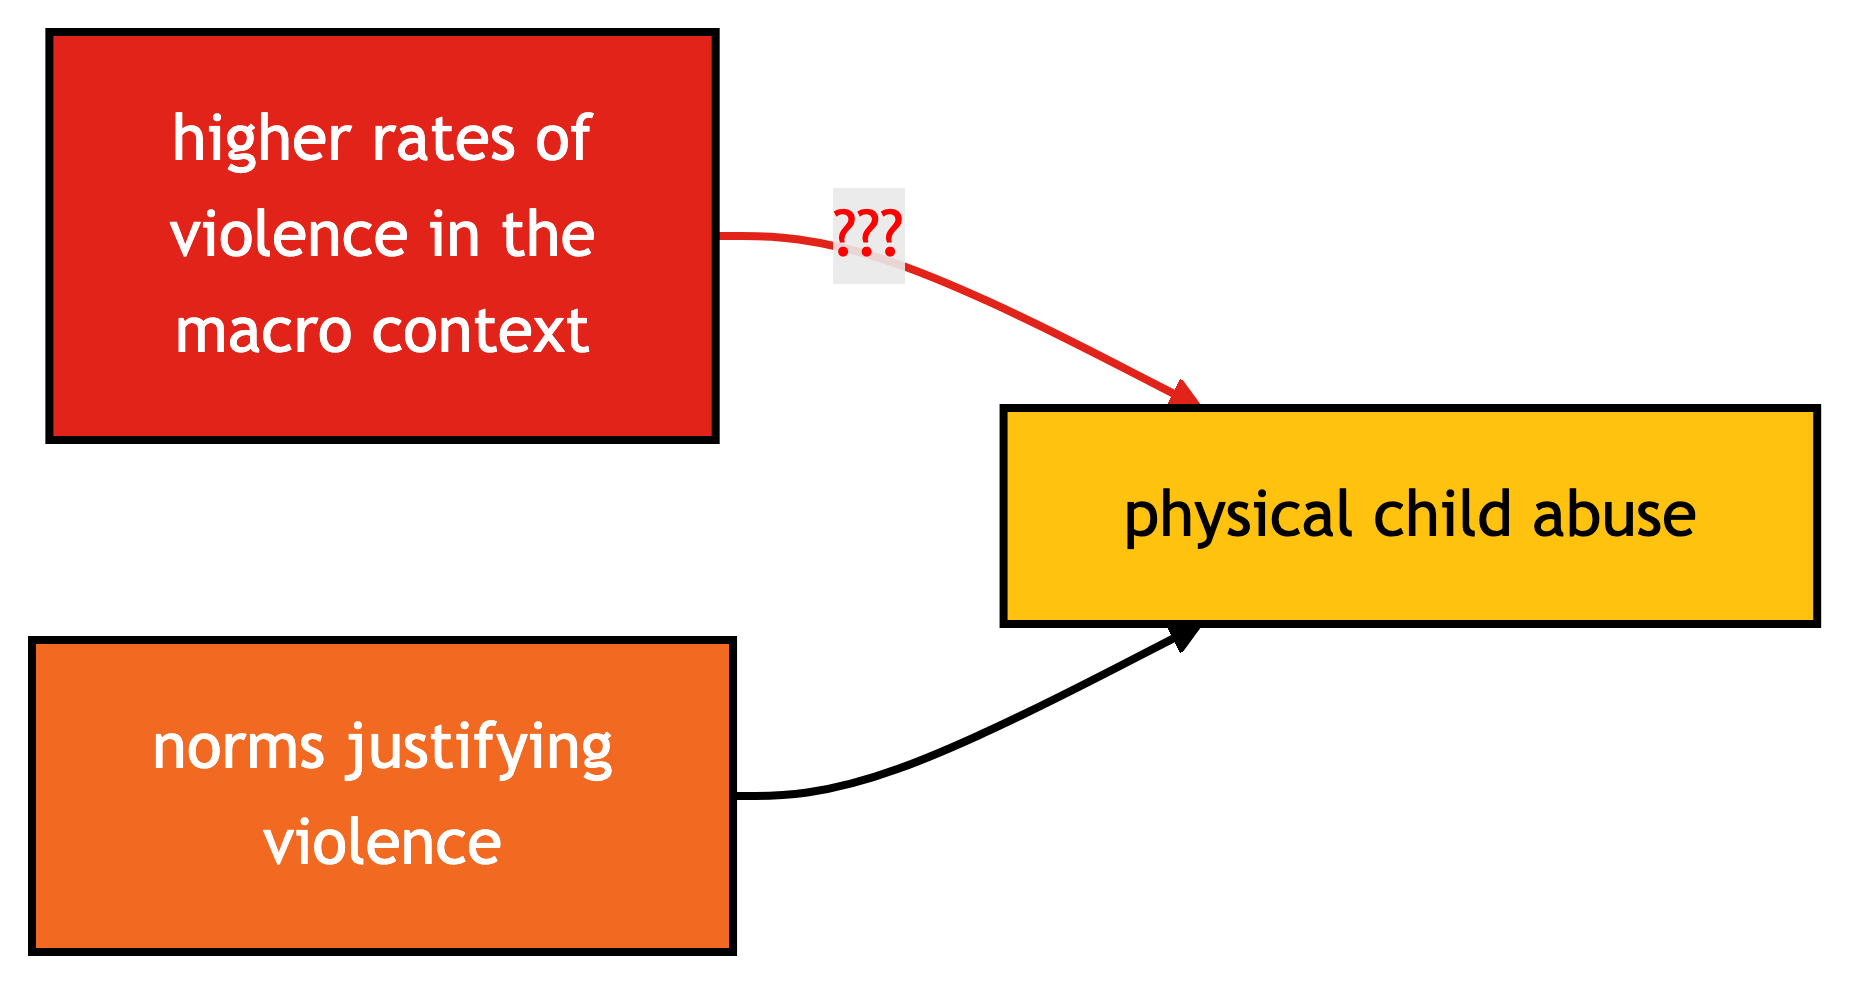
\includegraphics[width=4.82in,height=2.56in]{spillover-of-violence_files/figure-latex/mermaid-figure-1.png}

We used data from 435,131 households with a reference child aged 1 to 17
years across 43 countries from rounds 4 and 5 of the UNICEF Multiple
Indicator Cluster Surveys.

\protect\phantomsection\label{cr-earth}
\begin{figure}

\centering{

\pandocbounded{
\includegraphics[keepaspectratio]{spillover-of-violence_files/figure-pdf/fig-2-1.pdf}}

}

\caption{\label{fig-2}Countries in UNICEF MICS Data}

\end{figure}%

We employed multilevel logistic regression models.

We estimated the factors associated with parental physical abuse.

We controlled for country-level violence---measured by rates of
terrorism and political conflict, homicide, and women's exposure to IPV

We also controlled for other covariates, including norms justifying
violence against women and children and socio-demographic factors.

We accounted for the country in which study participants lived.

\protect\phantomsection\label{cr-analysis}
\begin{figure}[H]

{\centering \pandocbounded{\includegraphics[keepaspectratio]{annotated-equation.png}}

}

\caption{Multilevel Logistic Regression}

\end{figure}%

Results indicated that higher levels of endorsement of IPV (OR = 1.024,
p \textless{} .001) and attitudes endorsing the use of physical
punishment with children (OR = 1.016, p \textless{} .05) were both
associated with higher odds of severe physical child abuse after
controlling for covariates.

\protect\phantomsection\label{cr-results1}
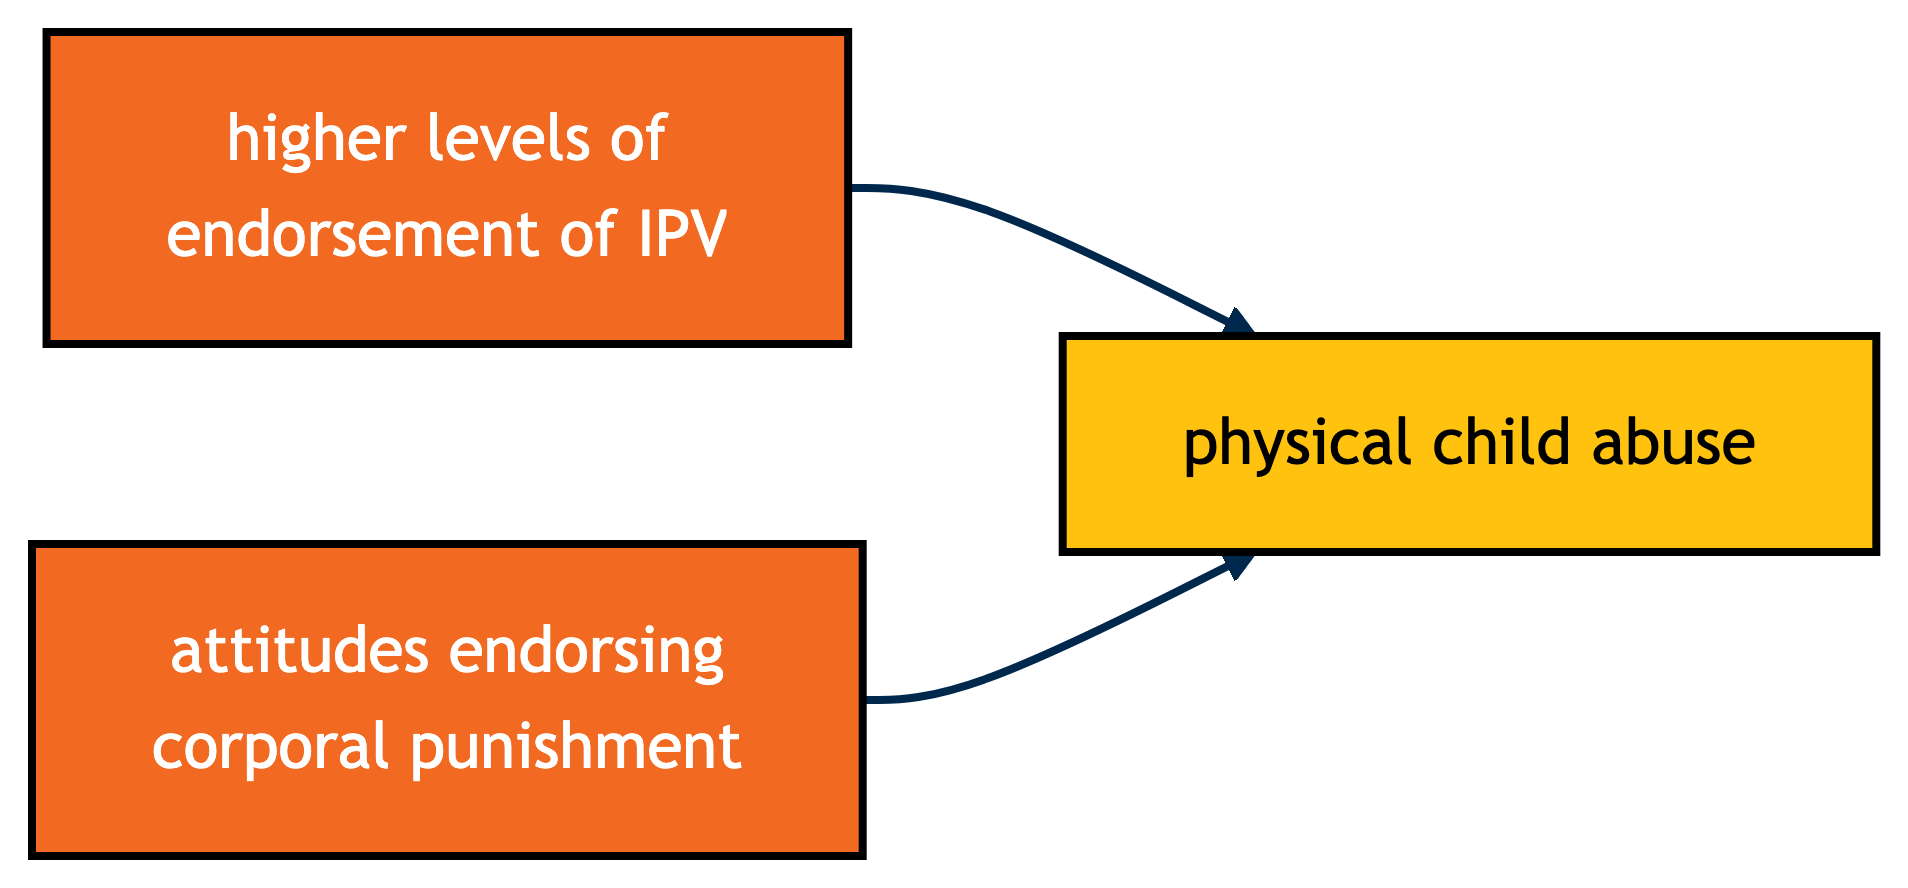
\includegraphics[width=4.97in,height=2.31in]{spillover-of-violence_files/figure-latex/mermaid-figure-4.png}

The association of terrorism and political violence with severe physical
abuse was mediated (statistically connected) by norms that legitimize
IPV (indirect b = 0.027, p = .005).

\protect\phantomsection\label{cr-results2}
\begin{Shaded}
\begin{Highlighting}[]
\NormalTok{spillover }\OtherTok{\textless{}{-}} \FunctionTok{read\_csv}\NormalTok{(}\StringTok{"spillover.csv"}\NormalTok{)}

\NormalTok{m }\OtherTok{\textless{}{-}} \FunctionTok{list}\NormalTok{(}
  \AttributeTok{l =} \DecValTok{50}\NormalTok{,}
  \AttributeTok{r =} \DecValTok{50}\NormalTok{,}
  \AttributeTok{b =} \DecValTok{100}\NormalTok{,}
  \AttributeTok{t =} \DecValTok{200}\NormalTok{,}
  \AttributeTok{pad =} \DecValTok{4}
\NormalTok{)}

\NormalTok{p\_spillover }\OtherTok{\textless{}{-}} \FunctionTok{plot\_ly}\NormalTok{(}\AttributeTok{data =}\NormalTok{ spillover, }
                       \AttributeTok{x =} \SpecialCharTok{\textasciitilde{}}\NormalTok{percentile, }
                       \AttributeTok{y =} \SpecialCharTok{\textasciitilde{}}\NormalTok{abuse, }
                       \AttributeTok{text =} \SpecialCharTok{\textasciitilde{}}\FunctionTok{paste}\NormalTok{(}\StringTok{"percentile of political violence and terrorism: "}\NormalTok{, }
\NormalTok{                                     percentile, }
                                     \StringTok{\textquotesingle{}\textless{}br\textgreater{}probability of abuse:\textquotesingle{}}\NormalTok{, }
\NormalTok{                                     abuse),}
                       \AttributeTok{hoverinfo =} \StringTok{\textquotesingle{}text\textquotesingle{}}\NormalTok{,}
                       \AttributeTok{marker =} \FunctionTok{list}\NormalTok{(}\AttributeTok{size =} \DecValTok{15}\NormalTok{,}
                                     \AttributeTok{color =} \StringTok{\textquotesingle{}\#E2231A\textquotesingle{}}\NormalTok{,}
                                     \AttributeTok{line =} \FunctionTok{list}\NormalTok{(}\AttributeTok{color =} \StringTok{\textquotesingle{}black\textquotesingle{}}\NormalTok{,}
                                                 \AttributeTok{width =} \DecValTok{2}\NormalTok{)),}
                       \AttributeTok{type =} \StringTok{\textquotesingle{}scatter\textquotesingle{}}\NormalTok{, }
                       \AttributeTok{mode =} \StringTok{\textquotesingle{}lines+markers\textquotesingle{}}\NormalTok{,}
                       \AttributeTok{height =} \DecValTok{700}\NormalTok{) }\SpecialCharTok{\%\textgreater{}\%}
  \FunctionTok{layout}\NormalTok{(}\AttributeTok{title =} \StringTok{\textquotesingle{}As political violence and terrorism increase, \textless{}br\textgreater{}so does the probability of physical abuse.\textquotesingle{}}\NormalTok{, }
         \AttributeTok{xaxis =} \FunctionTok{list}\NormalTok{(}\AttributeTok{title =} \StringTok{"percentile of political violence and terrorism"}\NormalTok{),}
         \AttributeTok{yaxis =} \FunctionTok{list}\NormalTok{(}\AttributeTok{title =} \StringTok{"probability of abuse"}\NormalTok{),}
         \AttributeTok{hoverlabel =} \FunctionTok{list}\NormalTok{(}\AttributeTok{bgcolor =} \StringTok{"white"}\NormalTok{),}
         \AttributeTok{margin =}\NormalTok{ m) }\SpecialCharTok{\%\textgreater{}\%} 
  \FunctionTok{config}\NormalTok{(}\AttributeTok{displayModeBar =} \ConstantTok{FALSE}\NormalTok{)}

\NormalTok{p\_spillover }\CommentTok{\# replay}
\end{Highlighting}
\end{Shaded}

\pandocbounded{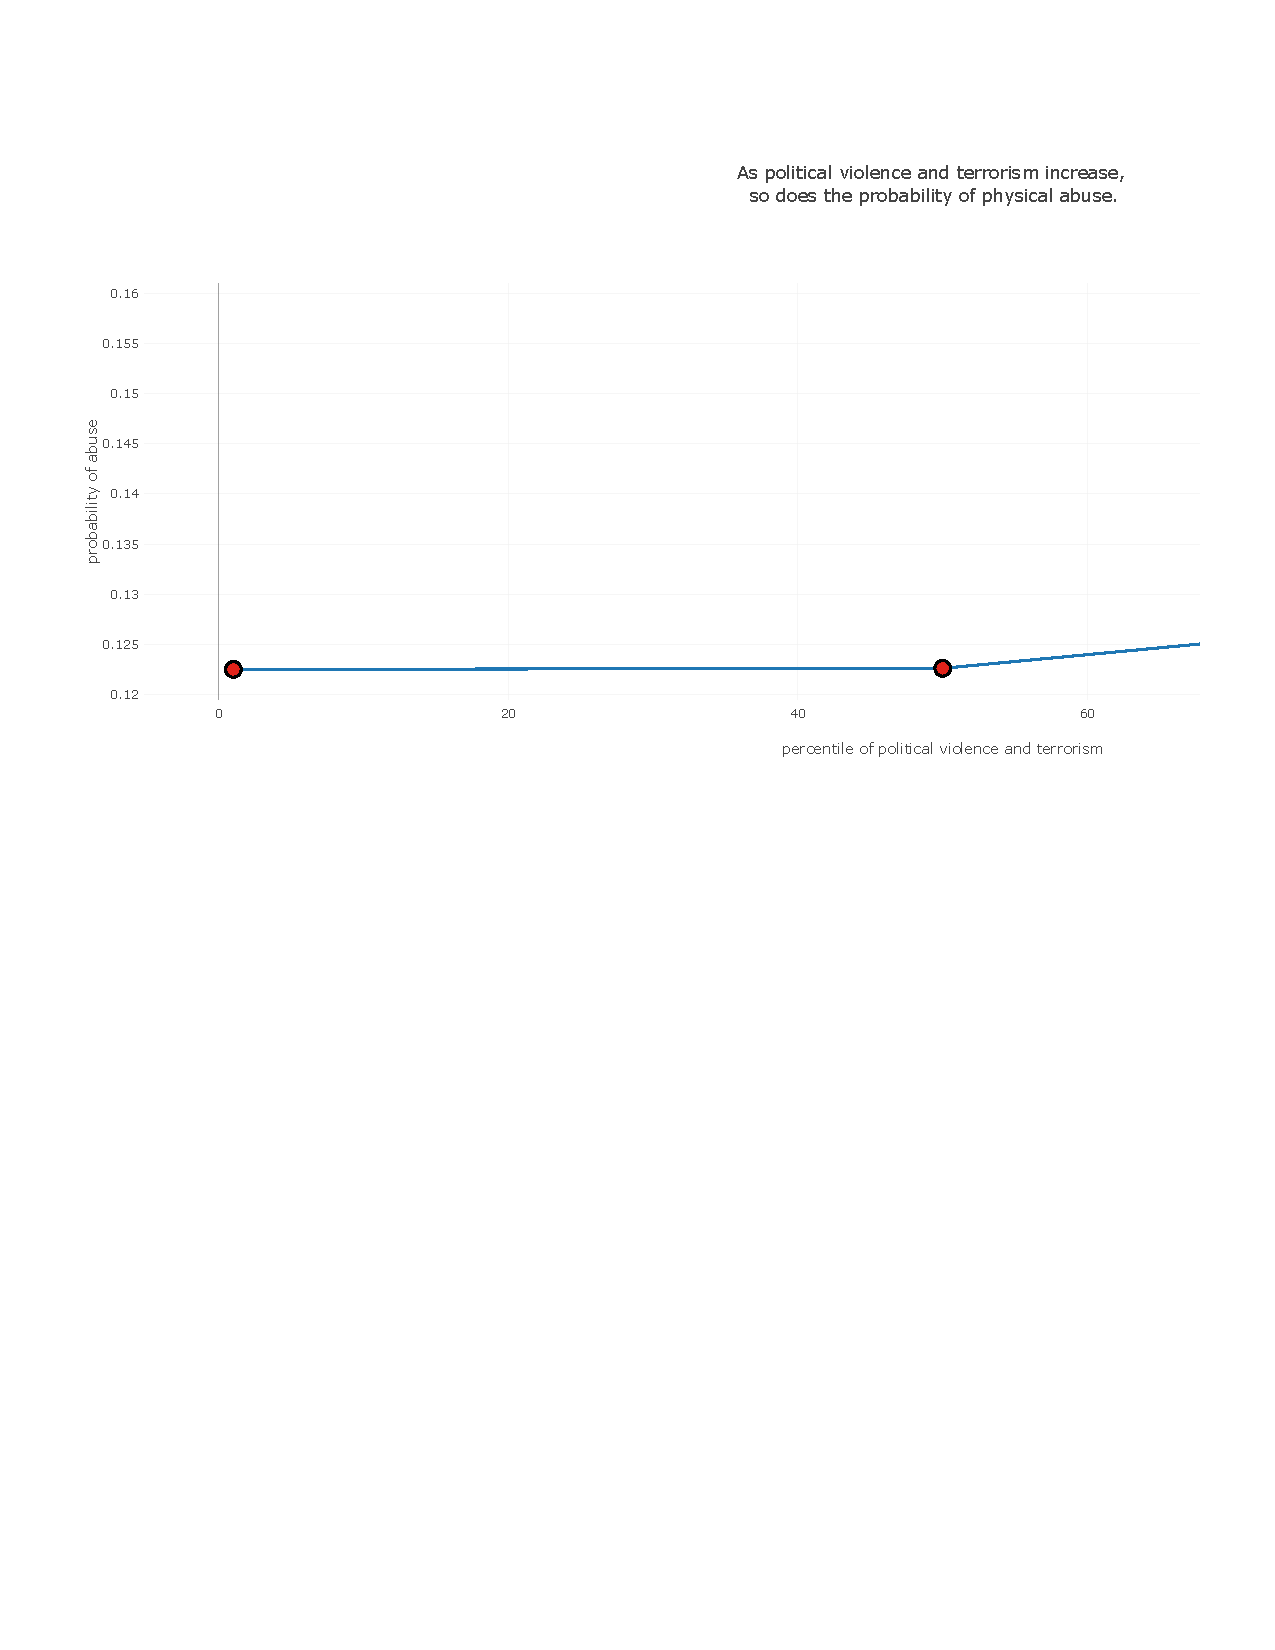
\includegraphics[keepaspectratio]{spillover-of-violence_files/figure-pdf/unnamed-chunk-6-1.pdf}}

Interventions aimed at reducing abusive parenting practices in LMICs may
benefit from efforts to reduce social norms that support violence
against women and children.

These interventions should be responsive to trauma-informed approaches
that recognize the effects of macro-level violence.

\protect\phantomsection\label{cr-interventions}
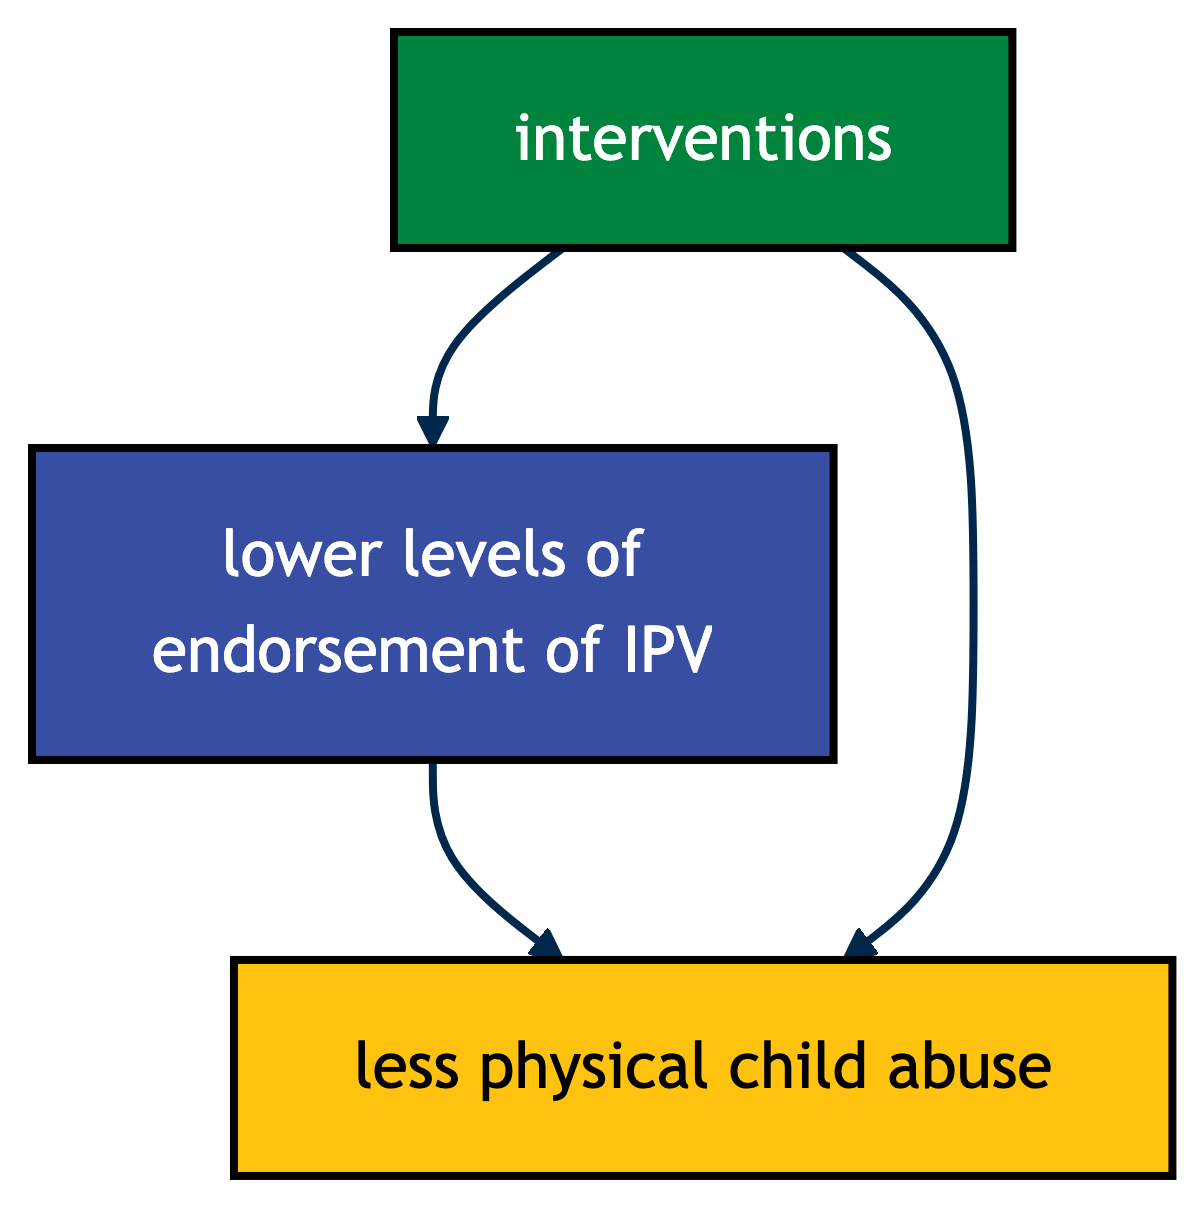
\includegraphics[width=3.14in,height=3.15in]{spillover-of-violence_files/figure-latex/mermaid-figure-3.png}

\protect\phantomsection\label{cr-interventions2}
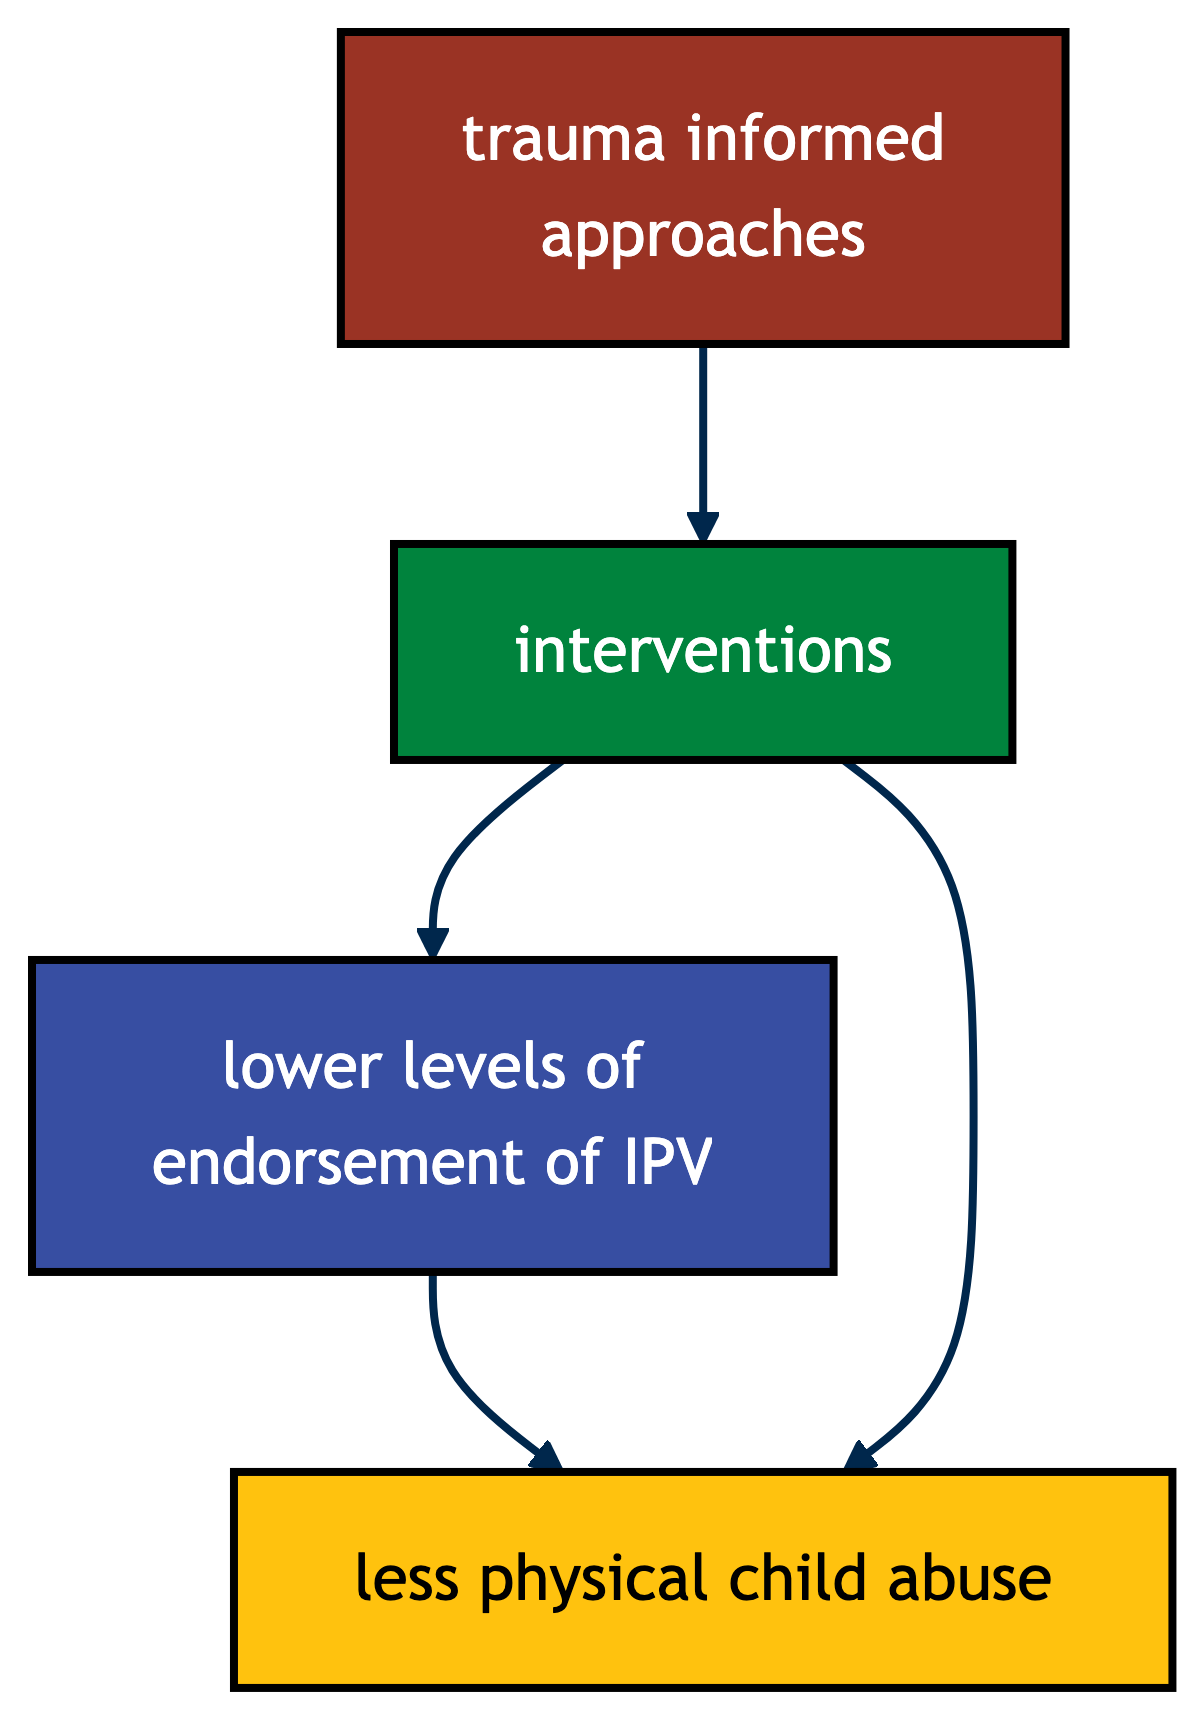
\includegraphics[width=3.14in,height=4.48in]{spillover-of-violence_files/figure-latex/mermaid-figure-2.png}

\protect\phantomsection\label{refs}
\begin{CSLReferences}{1}{1}
\bibitem[\citeproctext]{ref-Ma2025}
Ma, Julie, Andrew Grogan-Kaylor, Kaitlin P. Ward, Elizabeth H. Boyle,
Olivia D. Chang, and Garrett T. Pace. 2025. {``Spillover of Macro-Level
Violence to Parental Physical Abuse of Children in Low- and
Middle-Income Countries.''} \emph{Child Abuse \& Neglect} 164 (June):
107468. \url{https://doi.org/10.1016/j.chiabu.2025.107468}.

\end{CSLReferences}



<div class= "page-columns page-rows-contents page-layout-article"><div class="social-share"><a href="https://www.linkedin.com/shareArticle?url=https://agrogan1.github.io/closeread/spillover-of-violence/spillover-of-violence.html&title=Spillover of Violence" target="_blank" class="linkedin"><i class="fa-brands fa-linkedin-in fa-fw fa-lg"></i></a>  <a href="mailto:?subject=Spillover of Violence&body=Check out this link:https://agrogan1.github.io/closeread/spillover-of-violence/spillover-of-violence.html" target="_blank" class="email"><i class="fa-solid fa-envelope fa-fw fa-lg"></i></a><a href="https://www.facebook.com/sharer.php?u=https://agrogan1.github.io/closeread/spillover-of-violence/spillover-of-violence.html" target="_blank" class="facebook"><i class="fab fa-facebook-f fa-fw fa-lg"></i></a><a href="https://reddit.com/submit?url=https://agrogan1.github.io/closeread/spillover-of-violence/spillover-of-violence.html&title=Spillover of Violence" target="_blank" class="reddit">   <i class="fa-brands fa-reddit-alien fa-fw fa-lg"></i></a><a href="javascript:void(0);" onclick="var mastodon_instance=prompt('Mastodon Instance / Server Name?'); if(typeof mastodon_instance==='string' &amp;&amp; mastodon_instance.length){this.href='https://'+mastodon_instance+'/share?text=Spillover of Violence https://agrogan1.github.io/closeread/spillover-of-violence/spillover-of-violence.html'}else{return false;}" target="_blank" class="mastodon"><i class="fa-brands fa-mastodon fa-fw fa-lg"></i></a><a href="https://bsky.app/intent/compose?text=https://agrogan1.github.io/closeread/spillover-of-violence/spillover-of-violence.html Spillover of Violence" target="_blank" class="bsky"><i class="fa-brands fa-bluesky"></i></a></div></div>


\end{document}
